\section{Simplicial Homology}

    An \emph{$n$-simplex}, denoted by $\Delta^n=[v_0,\dots,v_n]$ is the smallest convex set in $\R^m$ containing $n+1$ points $v_0,\dots,v_n$ that do not lie in a hyperplane of dimension less than $n$. Or, equivalently, such that $v_1-v_0,\dots,v_n-v_0$ are linearly independant. The $n+1$ point $v_0,\dots,v_n$ are the \emph{vertices} of the $n$-simplex. A by-product of our ordered notation for the vertices of a simplex is that it determines an orientation for the edges $[v_i,v_j]$ according to the increasing subscripts. The \emph{faces} of an $n$-simplex are all the sub-simplices that can obtained by removing vertices of the original simplex. The order of the vertices of the smaller simplices is taken to be same than in the original $n$-simplex. 
    
    Let us now put some simplices together. If $X$ be a topological space, then a \emph{simplicial complex structure} $\Delta$ on $X$ is a collection $\Delta=\{\sigma_\alpha\}$ of continuous maps $\sigma_\alpha:\Delta^{n(\alpha)}\to X$ called \emph{characteristic maps} such that
    \begin{enumerate}[label=\roman*)]
        \item $\sigma_\alpha|_{e^{n(\alpha)}}$ is injective and that for all $x\in X$ there exists $\alpha$ such that $x\in\Im(\sigma_\alpha|_{e^{n(\alpha)}})$,
        \item the restriction of any map $\sigma_\alpha$ to a face of $\Delta^n$ is another $\sigma_\beta$,
        \item for any subset $A\subseteq X$, $A$ is open if and only if $\sigma^{-1}_{\alpha}(A)$ is open in $\Delta^n$ for all $\alpha$,
    \end{enumerate}
    where $\Delta^n$ is an $n$-simplex and $e^n$ is the interior of $\Delta^n$. 

    Given a simplicial complex structure $\Delta$ on $X$, $n$-chains are finite formal sums
    \begin{equation}
        \sum_\alpha n_\alpha \sigma_\alpha(e^{n(\alpha)})
    \end{equation}
    with coefficient $n_\alpha\in\Z$. We denote by $\Delta_n(X)$ the set of all $n$-chains, it is a free abelian group.

    For a general simplicial complex structure on $X$, we define a \emph{boundary homomorphism} $\p_n:\Delta_n(X)\to\Delta_{n-1}(X)$ by its action on the basis elements:
    \begin{equation}
        \p_n(\sigma_\alpha)=\sum_i(-1)^i\sigma_\alpha|_{[v_0,\dots,\hat{v_i},\dots,v_n]}.
    \end{equation}
    In particular, homomorphism here means that this maps are linear. We can note that the right side of this equation does indeed lies in $\Delta_{n-1}(X)$ since each restriction $\sigma_\alpha|_{[v_0,\dots,\hat{v_i},\dots,v_n]}$ is the characteristic map of an $(n-1)$-simplex of $X$. The most important property of those maps is that $\p_{n}\circ\p_{n+1}=0$ (symbolically $\p^2=0$), meaning that $\Im\p_{n+1}\subset\Ker\p_n$. We can then form a sequence of homomorphisms of abelian groups
    \begin{equation}
        \dots\to \Delta_{n+1}(X)\xrightarrow[]{\p_{n+1}}\Delta_n(X)\xrightarrow[]{\p_{n}}\Delta_{n-1}(X)\to\dots\to\Delta_1(X)\xrightarrow[]{\p_{1}}\Delta_0(X)\to 0
    \end{equation}
    $\Im\p_{n+1}\subset\Ker\p_n$ for each $n$. Chains of homomorphisms satisfying this property are called \emph{chain complex}. We have extended the chain at the end with $\p_0=0$ such that this property is also true at the ends. Elements of $\Ker\p_n$ are called \emph{$n$-cycles} and elements of $\Im\p_{n+1}$ are called \emph{$n$-boundaries}. Note that they are each elements of $\Delta_n(X)$, hence the notation. 
    \begin{examp*}
        If we consider a triangle withe vertices $A,B$ and $C$, we can put a simplicial complex structure on it consisting of one $2$-simplex ($u=[A,B,C]$), three 1-simplices ($a=[A,B],b=[B,C],c=[C,A]$) and three $0$-simplices ($A,B,C$). We can see that
        \begin{equation}
            \p_2(u)=[B,C]-[A,C]+[A,B] = a+b+c.
        \end{equation} 
        So we get that $a+b+c$ is a $1$-boundary. However, we see that
        \begin{equation}
            \p_1(a+b+c)=B-A+C-B+A-C=0
        \end{equation}
        so it is also a $1$-cycle.
    \end{examp*}
    The fact that image of each map lies the kernel of the next map means that any boundary is also a cycle. As illustrated by the previous example. We can wonder what are the cycles that are not boundaries of any higher-dimensional simplicial complex. This set is precisely the quotient space
    \begin{equation}
        H_n(X)=\frac{\Ker(\p_n)}{\Im\p_{n+1}}.
    \end{equation}
    It naturally inherits a group structure and is called the $n$th \emph{Homology group} of $X$. The elements of this space are equivalence classes (cosets of $\Im\p_{n+1}$) of $n$-cycles where two cycles are considered equivalent if they only differ by a boundary, i.e. if their formal difference is a boundary. These equivalence classes are called \emph{homology classes}.

    \begin{examp*}
        Let us give some useful examples of Homology groups for various topological spaces:
        \begin{itemize}
            \item the Homology groups of $\R^n$ are all trivial therefore $\chi=0$.
            \item the non-trivial Homology groups of the $n$-sphere are $H_0(S^n)=H_n(S^n)=\Z$ therefore $\chi=(-1)^n-1$
            \item the only non-trivial Homology group of the $n$-ball is $H_0(B^n)=\Z$ therefore $\chi=1$.
            \item the non-trivial Homology groups of the $2$-torus are $H_0(T)=H_2(T)=\Z$ and $H_1(T)=\Z^2$ therefore $\chi=(1+x)^2$.
            \item the non-trivial Homology groups of the complex projective space are $H_{0\leq 2k\leq 2n}(\C\P^n)=\Z$.
            \item the only non-trivial Homology groups of any Riemann surface of genus $g$ are $H_0=\Z, H_1=\Z^{2g}$ and $H_2=\Z$, such that $\chi=2-2g$.
        \end{itemize}
    \end{examp*}
    Let us make a comment on the zeroth homology group. Since $\Ker\p_0=\Delta_0$ by definition, all elements of $\Delta_0$ (i.e. every point of $X$) are $0$-cycles and $H_0(X)$ is the set of $0$-cycles that are not the boundary of any chain of $1$-simplices. Since any linear combination of $0$-simplices (i.e. point) can be seen as the boundary the $1$-simples that joins them, we can see that all points that can be joined by a path are equivalent. For a topological space $X$ where all points can be connected by a path this means that the zeroth homology group is necessarily $H_{0}(X)=\{nA|a\in\Z\}\cong\Z$, where $A$ any point in $X$. More generally, we can conclude that the number of copies of $\Z_n$ in $H_0(X)$ is the number of path-connected components of $X$.

    For a graph $\Gamma$, we can understand from our previous discussions that the only non-trivial homology groups are going to be $H_0(\Gamma)=\Z\times\dots\times\Z$ where the number of copies is the number of connected components and $H_1(\Gamma)=\Z\times\dots\times\Z$ where the number of copies is the number of ``irreducible'' loops.

    The $n$th simplicial homology group of a topological space $X$ with a complex simplicial structure $\Delta$ is always of the form
    \begin{equation}
        H^\Delta_n(X)=\underbrace{\Z\times\Z}_{b_n}\oplus\Z_{q_1}\times\dots\times\Z_{q_s}.
    \end{equation}
    $b_n$ are the Betti numbers. The \emph{Poincaré polynomial} is
    \begin{equation}
        P_X(x)=\sum_{i\geq 0}b_ix^i
    \end{equation}
    and the Euler characteristic of $X$ is given by $P_X(-1)$. Recall that the Euler characteristic is also given by $\chi=2-2g-b-c$, $g$ being the genus, $b$ the number of topological boundaries and $c$ the number of crosscaps.

    Note that the homology that we considered is with coefficients in $\Z$, i.e. we started with simplicial chains with coefficients in $\Z$. We can however also consider coefficients in $\R$, in $\C$ or in any ring. In those case however we can easily lose the information about torsion. For example $\Z/2\Z=\Z_2$ is non trivial but since $2\R=\R$, $\R/2\R=\{0\}$.

\section{Spacetime geometry: ALE space and orbifolds}\label{app:spacetimegeom}

    Asymptotically locally euclidean (ALE) spaces are a particularly interresting choice of string background to probe with branes for mainly four reasons
    \begin{enumerate}[label=(\roman*)]
        \item they are the resolution (blow-ups) of orbifolds
        \item there are completely classified: they fall in the ADE classification
        \item they only break half of the supersymmetry
        \item they are non-compact therefore we can study them for self-dual type II theory. \todo{Why is that ?}
    \end{enumerate}
    Mathematically, an ALE space is complete riemannian $n$-manifold $M$ such that there exists a compact set $K\subset M$ such that $M\backslash K$ is diffeomorphic to $(\R^n\backslash B_0(R))/G$, where $R\in\R^+_0$ is a radius and $G\subset\O(n)$ a subgroup. Additionally, it is asked that the pulled back metric on $\R^n\backslash B_0(R)$ tends to the euclidean flat metric at infinity.

    If one considers string theory an the orbifold $\R^4/\Gamma$ where $\Gamma$ is a finite sub group of $\SU(2)$, massless states appear from the twisted sector. They are precisely the moduli needed the deform the theory to the one with smooth spacetime, i.e. the resolution of the orbifold. In that sense, is said that the strings know about the metric ALE space and that it is said that strings resolve the singularity. The metric of the ALE space can be recovered if the lagrangian of the resulting field theory is explicitely know, such as for the Wess-Zumino-Witten model. However, it is often not the case.



        

\section{Determinantal varieties as transverse spaces}

    \subsection{Basic properties of determinantal varieties}  

            A \emph{determinantal variety} (DV) is a space of matrices with a given upper bound on their ranks. More precisely, given $m,n$ and $r<\min(m,n)$, the DV $Y_r$ of the field $K$ is the set of $m\times n$ matrices over $K$ with rank lower or equal to $r$:
            \begin{equation}
                Y_r\equiv\{M\in M_{m\times n}(K)|\rank M\leq r\}.
            \end{equation}
            Recall that a $k$-minor is the determinant of a $k\times k$ sub-matrix and that the rank of a matrix is equal to the biggest integer such that there is a non-vanishing minor of that size. Imposing $\rank M\leq r$ is therefore equivalent to the vanishing of its $(r+1)\times (r+1)$ minors, as it also implies tha vanishing of the biggest minors. This naturally qualifies $R_r$ as affine varieties embedded in $K^{mn}$. 
            
            Let us denote by $X=(x_{ij})$ an arbitrary $m\times n$ matrix. The independent entries $x_{ij}$ are affine coordinates. The $(r+1)\times(r+1)$ minors are therefore homogeneous polynomials of degree $r+1$. The \emph{determinantal ideal} $I_{r+1}(X)$ is the ideal of $k[X]$ generated by these polynomials. The cooridnate ring is 
            \begin{equation}
                R=k[X]/I_{r+1}(X)
            \end{equation}
            Homogeneity the polynomials implies that $Y_r$ can equivalently be seen as a projective variety in $\bbA^{mn-1}$.

        \subsubsection{Computing the dimension}
            
            Let us compute the dimension of $Y_r$ seen as an affine variety. We consider the space $\bbA^{mn}\times\textbf{Gr}(r,m)$, where $\textbf{Gr}(r,m)$ is the Grassmannian of $r$-planes in an $m$-dimensioanl vector space. Let us define the subsapce
            \begin{equation}
                Z_r\equiv\{(A,W)|Ax\in W\text{ for all } x\in\bbA^{n}\}.
            \end{equation}
            $Y_r$ and $Z_r$ are birationaly equivalent so $\dim Y_r=\dim Z_r$. We want to compute $Z_r$. First we notice that $Z_r$ is a vector bundle over $\textbf{Gr}(r,m)$ and we denote it by $Z_r\xrightarrow[]{\pi_1}\textbf{Gr}(r,m)$. Now, over the Grassmannian $\textbf{Gr}(r,m)$, there is a tautologial vector bundle that we denote by $E_{\textbf{Gr}}\xrightarrow[]{\pi_2}\textbf{Gr}(r,m)$ whose fibers are $\pi^{-1}_2(W)=W\cong\R^r$. Finally, $K^m$ can also be seen as a vector bundle, with fibers $\R^m$. We denote it by $E_{K^n}\xrightarrow[]{\pi_3}K^n$. From $E_{\textbf{Gr}}$ and $E_{K^n}$, we can construct\footnote{Recall that if $E$ and $F$ are vector bundles over $X$, then we can construct a new vetor bundle over $X$, called the Hom-bundle and denoted $\Hom(E,F)$, by defining the fiber over $x\in X$ to be $\Hom(E_x,F_x)$.} the vector bundle $\Hom(E_{\textbf{Gr}},E_{K^n})\xrightarrow[]{\pi_4}\textbf{Gr}(r,m)$. This vector bundle has the same base space and its fibers are $\Hom(\R^m,\R^r)$ which are exactly the same as the ones of $Z_r$. So the two vector bundles are isomorphic:
            \begin{equation}
                Z_r\cong\Hom(E_{\textbf{Gr}},E_{K^n}).
            \end{equation}
            Finally, since the fibers of $\Hom(K^n,E_{\textbf{Gr}})$ have dimension $nr$, we find
            \begin{equation}
                \dim Z_r = \dim\Hom(K^n,E_{\textbf{Gr}}) = \dim\textbf{Gr}(r,m)+nr = r(m-r)+nr.
            \end{equation}
            Finally, we conclude that $Y_r$ is a affine variety of dimension $r(m-r)+nr$.

            \begin{table}[H]
                \centering
                $
                \begin{array}{|c|c|c||c|}
                    \hline
                    m & n & r & \dim_\C Y_r \\ \hline
                    2 & 2 & 1 & 3 \\ \hline
                    3 & 2 & 1 & 4 \\ \hline
                    3 & 3 & 1 & 5 \\ \hline
                    3 & 3 & 2 & 8 \\ \hline
                    4 & 2 & 1 & 5 \\ \hline
                    4 & 3 & 1 & 6 \\ \hline
                    4 & 3 & 2 & 10 \\ \hline
                    4 & 4 & 1 & 7 \\ \hline
                    4 & 4 & 2 & 12 \\ \hline
                    4 & 4 & 3 & 15 \\ \hline
                \end{array}
                $
            \end{table}

        \subsubsection{Singularity}
        
            Determinantal varieties are singular and possess non-commutative resolutions. $Y_r$ is singlar and the singular locus is contained in the subset of matrices with rank strictly lower than $r$. $Z_r$ is a resolution (over the open set of matrices with rank exactly $r$, this map is an isomorphism), it is called the \emph{Springer desingularization} of $\text{Spec}R$.

        \subsubsection{Action and syzygies}

            $Y_r$ naturally acts on $G=\GL(m,K)\times\GL(n,K)$

        \subsection{Young's lattice}

            \emph{Young's lattice} is a lattice $Y$ formed by all integer partitions ordered by inclusion of their Young tableau. It is generally used to to describe the irreducible representation sof the symmetric group\footnote{Two permutations of $S_n$ are equivalent if and only they have they have the same number of cycles of the same sizes. Therefore, the quivalence classes of the symmetric group $S_n$ are parametrized by the partitions of $n$, i.e. by Young diagrams.} $S_n$ together with their branching properties. Conventionnally, Young's lattice is depicted in a Hasse diagram, i.e. with element of the same rank shown at the same height and with links such that the descendance of two elements is the union and the parent is the intersection.

            \begin{figure}[H]
                \centering
                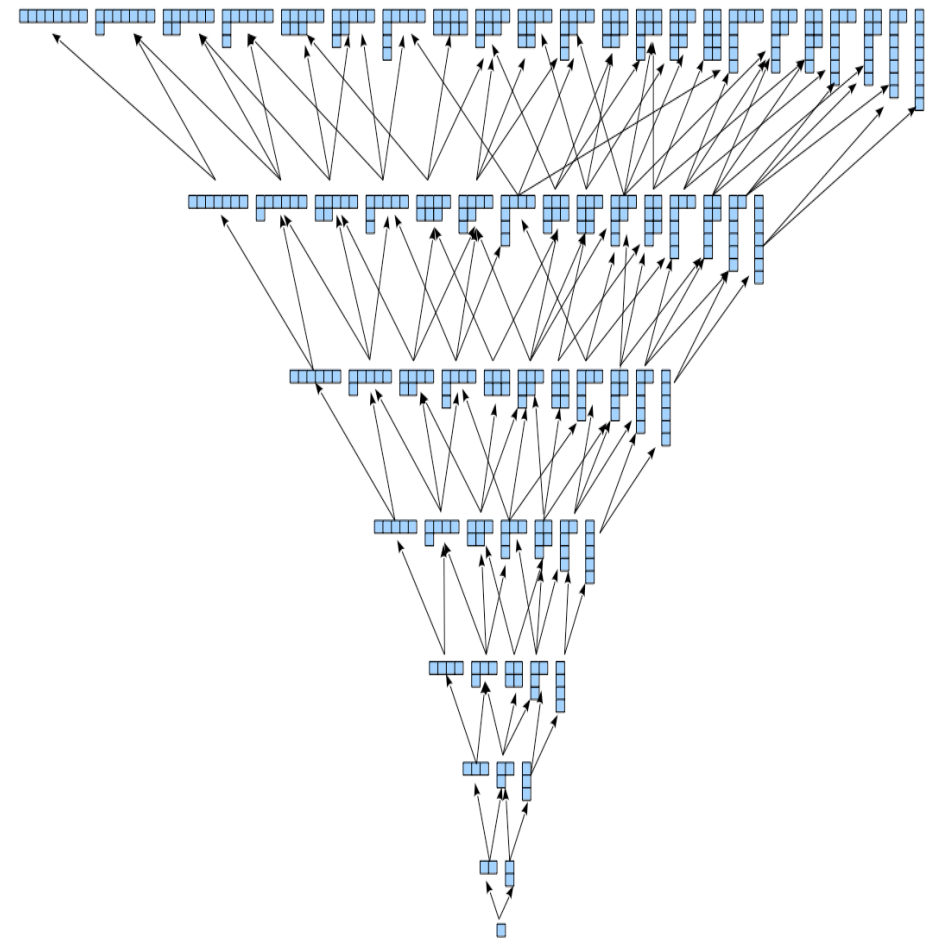
\includegraphics[scale=0.45]{Pictures/youngslattice.png}
                \caption{Young's lattice.}
            \end{figure}

            Young's lattice possess the folling symmetry: the partition $n+n-1+\dots2+1$ of the $n$th triangular number has a Young diagram that looks like a staircase. If we now only keep the elements whose hull is contained in this staircase, we get a subset of Young's lattice. When rank-embedded, this subset clearly has the expected bilateral symmetry of Young's lattice but also a rotational symmetry, which appear more clearly if we move away from this rank-embedding. The rotation group of order $n+1$ acts on this poset\footnote{Partially ordered set.}. Since it has both a bilateral and a rotational symmetry it must also have a dihedral symmetry and, indeed, the dihedral group $\D_{n+1}$ acts faithfully on this set.

            \begin{figure}[H]
                \centering
                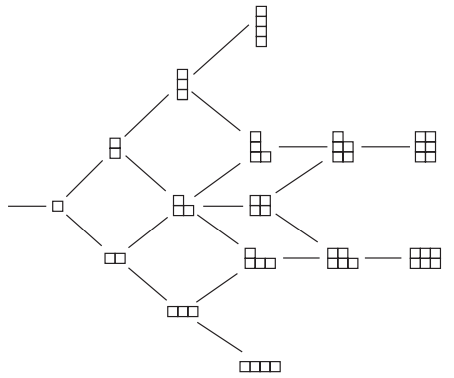
\includegraphics[scale=0.45]{Pictures/suter1.png}
                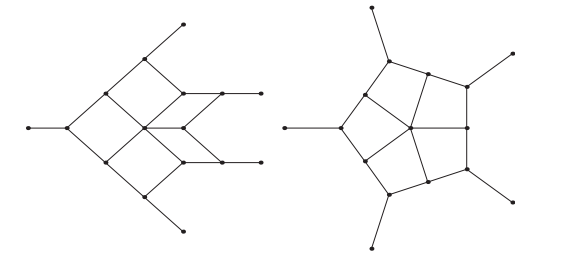
\includegraphics[scale=0.45]{Pictures/suter2.png}
                \caption{Example of dihedral symmetry for $n=4$.}
            \end{figure}

\section{Some derivations}

    \subsection{Invariant configurations for $\C\times\C^2/2\D_n$}\label{app:invconfDn}

        \subsubsection{Gauge field}

            To find the invariant configurations of the gauge group, we use use the bi-index notation and split the sub-blocks of $A_\mu$ in four categories depending on the dimensionality of the representations that they transform in. Note that it is only necessary to check the invariance under the two generators of $2\D_n$ to ensure invariance under the whole group.
            \begin{itemize}
                \item components $A_{\mu;a\alpha_a,b\beta_b}$ are $1\times 1$ blocks that transform as $A_{\mu;a\alpha_a,b\beta_b}\mapsto\sigma_a(\gamma)A_{\mu;a\alpha_a,b\beta_b}\sigma_b(\gamma)^{-1}$. It follows that only the component with $a,b=0,1$ or $a,b=2,3$ can be non-zero to have invariance under $A$. For invariance under $B$, we find that only the component with $a,b=0,2$ or $a,b=1,3$ can be non-zero if $n$ is even and only the component with $a=b$ if $n$ is odd. In conclusion, the invarint configuration under $A$ and $B$ are of the form
                \begin{equation}
                    (A_{\mu;ab})=\begin{bmatrix}
                        \times & 0 & 0 & 0 \\
                        0 & \times & 0 & 0 \\
                        0 & 0 & \times & 0 \\
                        0 & 0 & 0 & \times
                    \end{bmatrix}
                \end{equation}
                regardless of the parity of $n$.
                \item components $A_{\mu;a\alpha_a,r\beta_r}$ are $1\times 2$ blocks that transform as $A_{\mu;a\alpha_a,r\beta_r}\mapsto\sigma_a(\gamma)A_{\mu;a\alpha_a,r\beta_r}\mu_r(\gamma)^{-1}$. More explicitely, each block is of the form $\begin{bmatrix} x_1 & x_2 \end{bmatrix}$ and transforms as
                \begin{equation*}
                    \begin{bmatrix} x_1 & x_2 \end{bmatrix}\mapsto\sigma_a(A)\begin{bmatrix} x_1\zeta^{-r}_{2n} & x_2\zeta^{r}_{2n} \end{bmatrix}
                \end{equation*}
                under the generator $A$. This never invariant unless $a=b=0$. There is no need to check the invariance under $B$ since all these component are already all zero.
                \item components $A_{\mu;r\alpha_r,a\beta_a}$ are $2\times 1$. The situation is exactly the samme as in the previous point: they must all vanish.
                \item components $A_{\mu;r\alpha_r,s\beta_s}$ are $2\times 2$ blocks that transform as $A_{\mu;r\alpha_r,s\beta_s}\mapsto\mu_r(\gamma)A_{\mu;r\alpha_r,s\beta_s}\mu_s(\gamma)^{-1}$. Generically speaking, an invariant block under $A$ must satisfy
                \begin{equation}
                    \begin{bmatrix}
                        \zeta^{r}_{2n} & 0 \\
                        0 & \zeta^{-r}_{2n}
                    \end{bmatrix}
                    \begin{bmatrix}
                        x_1 & x_2 \\
                        x_3 & x_4
                    \end{bmatrix}
                    \begin{bmatrix}
                        \zeta^{-s}_{2n} & 0 \\
                        0 & \zeta^{s}_{2n}
                    \end{bmatrix}=
                    \begin{bmatrix}
                        x_1\zeta^{r-s}_{2n} & x_2\zeta^{r+s}_{2n} \\
                        x_3\zeta^{-r-s}_{2n} & x_4\zeta^{-r+s}_{2n}
                    \end{bmatrix}=
                    \begin{bmatrix}
                        x_1 & x_2 \\
                        x_3 & x_4
                    \end{bmatrix}.
                \end{equation}
                There are two possibilities to have non-vanishing component: $\zeta^{r-s}_{2n}=1$ and $x_2=x_3=0$ or $\zeta^{r+s}_{2n}=1$ and $x_1=x_4=0$ but the latter is actually not possible since $r,s=1,\dots,n-1$. To we find that the blocks must be of the form
                \begin{equation}
                    A_{\mu;r\alpha_r,s\beta_s}=
                        \begin{bmatrix}
                            \times & 0 \\
                            0 & \times
                        \end{bmatrix}
                \end{equation}
                if $r=s$ and vanishing otherwise. For invariance under $B$, a blocks must satisfy
                \begin{equation}
                    \begin{bmatrix}
                        0 & -1 \\
                        1 & 0
                    \end{bmatrix}
                    \begin{bmatrix}
                        x_1 & x_2 \\
                        x_3 & x_4
                    \end{bmatrix}
                    \begin{bmatrix}
                        0 & -1 \\
                        1 & 0
                    \end{bmatrix}=
                    \begin{bmatrix}
                        -x_4 & x_3 \\
                        x_2 & -x_1
                    \end{bmatrix}=
                    \begin{bmatrix}
                        x_1 & x_2 \\
                        x_3 & x_4
                    \end{bmatrix}.
                \end{equation}
                which is only possible if $x_1-x_4$ and $x_2=x_3$. Finally, we find that invariance under $A$ and $B$ imposes the block to be of the form
                \begin{equation}
                    A_{\mu;r\alpha_r,s\beta_s}=
                        \begin{bmatrix}
                            x & 0 \\
                            0 & -x
                        \end{bmatrix}
                \end{equation}
                if $r=s$ and vanishing otherwise.
            \end{itemize}
            The invariant gauge field configurations were found to be of the form
            \begin{equation}
                A_\mu=
                {\tiny
                \left[
                \begin{array}{*{20}c}
                    \times & 0 & 0 & 0 & & & & & & \cdots & 0 \\
                    0 & \times & 0 & 0 & & & & & & & \\
                    0 & 0 & \times & 0 & & & & & & & \\
                    0 & 0 & 0 & \times & & & & & & & \\
                    & & & & x_1 & 0 & & & & & \\
                    & & & & 0 & -x_1 & & & & & \\
                    & & & & & & x_2 & 0 & & & \\
                    & & & & & & 0 & -x_2 & & & \\
                    \vdots & & & & & & & & \ddots & & \vdots \\
                    & & & & & & & & & x_{n-1} & 0 \\
                    0 & & & & & & & & & 0 & -x_{n-1}
            \end{array}
            \right]}\label{eq:invformAmuDn}
            \end{equation}
            where each entry $(i,j)$ is an arbitrary block of size $N_i\times N_j$.

        \subsubsection*{Scalar fields}

            For the real scalar fields $X^m$, we need the action of $2\D_n$ on $\C^3$:
            \begin{equation}
                \begin{bmatrix}
                    z_1\\z_2\\z_3
                \end{bmatrix}\overset{A}{\longmapsto}
                \begin{bmatrix}
                    1 & 0 & 0 \\
                    0 & \zeta_{2n} & 0 \\
                    0 & 0 & \zeta^{-1}_{2n}
                \end{bmatrix}
                \begin{bmatrix}
                    z_1\\z_2\\z_3
                \end{bmatrix},\qquad
                \begin{bmatrix}
                    z_1\\z_2\\z_3
                \end{bmatrix}\overset{B}{\longmapsto}
                \begin{bmatrix}
                    1 & 0 & 0 \\
                    0 & 0 & i \\
                    0 & i & 0
                \end{bmatrix}
                \begin{bmatrix}
                    z_1\\z_2\\z_3
                \end{bmatrix}.\label{eq:RsymDn}
            \end{equation}
            The partitionning of $X^m$ is similar to $A_\mu$. The additional difficulty is come from R-symmetry. Since it acts differently on the different components, we have the study themalmost one by one.
            \begin{itemize}
                \item the fields $X^0$ and $X^1$ are left untouched by R-symmetry, meaning that the invariant configurations have the same form than the gauge field, i.e. \eqref{eq:invformAmuDn}.
                \item $X^{2,3}_{a\alpha_a,b\beta_b}$ transforms under $A$ as $X^{2,3}_{a\alpha_a,b\beta_b}\mapsto \xi_{2n}\sigma_a(A) X^{2,3}_{a\alpha_a,b\beta_b}\sigma_b(A)^{-1}$. The only configurations that are left invariant are therefore the ones such that $ \xi_{2n}\sigma_a(A) \sigma_b(A)^{-1}=1$, which is never the case. So $X^{2,3}_{a\alpha_a,b\beta_b}=0$ for all $a,b=0,\dots,3$.
                \item $X^{2,3}_{a\alpha_a,k\beta_k}$ transforms under $A$ as $X^{2,3}_{a\alpha_a,k\beta_k}\mapsto \xi_{2n}\sigma_a(A) X^{2,3}_{a\alpha_a,k\beta_k}\mu_k(A)^{-1}$. More explicitely, if we denote a block$X^{2,3}_{a\alpha_a,k\beta_k}$ by $\begin{bmatrix} x_1 & x_2 \end{bmatrix}$, we get
                \begin{equation}
                    \begin{bmatrix}
                        \xi^{k+1}_{2n}\sigma_a(A) x_1 & \xi^{-k+1}_{2n}\sigma_a(A) x_2
                    \end{bmatrix}=
                    \begin{bmatrix}
                        x_1 & x_2
                    \end{bmatrix}
                \end{equation}
                therefore we can have $x_1\neq0$ iff $\sigma_a(A)=-1$(i.e. $a=2,3$) and $k=n-1$, and we can have $x_1\neq0$ iff $\sigma_a(A)=1$(i.e. $a=0,1$) and $k=1$.
                \item $X^{2,3}_{k\alpha_k,b\beta_b}$ transforms under $A$ as $X^{2,3}_{k\alpha_k,b\beta_b}\mapsto \xi_{2n}\mu_k(A) X^{2,3}_{k\alpha_k,b\beta_b}\sigma_a(A)^{-1}$. Similarly to the previous case, we can write the blocks $X^{2,3}_{k\alpha_k,a\beta_a}$ as $\begin{bmatrix} x_1 \\ x_2 \end{bmatrix}$, we get
                \begin{equation}
                    \begin{bmatrix}
                        \xi^{k+1}_{2n}\sigma_a(A) x_1 \\ \xi^{-k+1}_{2n}\sigma_a(A) x_2
                    \end{bmatrix}=
                    \begin{bmatrix}
                        x_1 \\ x_2
                    \end{bmatrix}
                \end{equation}
                therefore the conditions are exactly the same: we can have $x_1\neq0$ iff $\sigma_a(A)=-1$(i.e. $a=2,3$) and $k=n-1$, and we can have $x_1\neq0$ iff $\sigma_a(A)=1$(i.e. $a=0,1$) and $k=1$.
                \item $X^{2,3}_{k\alpha_k,l\beta_l}$ transforms under $A$ as $X^{2,3}_{k\alpha_k,l\beta_l}\mapsto \xi_{2n}\mu_k(A) X^{2,3}_{k\alpha_k,l\beta_l}\mu_l(A)^{-1}$. Again, we can write the blocks $X^{2,3}_{k\alpha_k,l\beta_l}$ as $\begin{bmatrix} x_1 & x_2 \\ x_3 & x_4 \end{bmatrix}$ and we get
                \begin{equation}
                    \begin{bmatrix} 
                        \zeta^{k-l+1}_{2n}x_1 & \zeta^{k+l+1}_{2n}x_2 \\
                        \zeta^{-k-l+1}_{2n}x_3 & \zeta^{-k+l+1}_{2n}x_4 
                    \end{bmatrix}=
                    \begin{bmatrix} 
                        x_1 & x_2 \\
                        x_3 & x_4 
                    \end{bmatrix}
                \end{equation}
                therefore, we can have
                \begin{itemize}
                    \item $x_1\neq0$ iff $l=k+1$,
                    \item $x_2\neq0$ iff $l=-k-1$ (not possible),
                    \item $x_3\neq0$ iff $l=-k+1$ (not possible),
                    \item $x_4\neq0$ iff $l=k-1$.
                \end{itemize}
                For $X^{4,5}_{i\alpha_i,j\beta_j}$, the reasonning is exactly the same but with the $R$-symmetry acting as $\zeta^{-1}_{2n}$ instead of $\zeta_{2n}$. After similar computations, we get that the components $X^{4,5}_{a\alpha_a,b\beta_b}$ must be all vanishing too and the components $X^{4,5}_{a\alpha_a,k\beta_k} = \begin{bmatrix} x_1 & x_2 \end{bmatrix}$ can have $x_1\neq0$ iff $a=0,1$ and $k=1$ and $x_2\neq0$ iff $a=2,3$ and $k=n-1$. The same goes for the components $X^{4,5}_{k\alpha_k,b\beta_b}=\begin{bmatrix}x_1\\ x_2\end{bmatrix}$ and, at last, for the components $X^{4,5}_{k\alpha_k,l\beta_l}=\begin{bmatrix} 
                    x_1 & x_2 \\
                    x_3 & x_4 
                \end{bmatrix}$, we find 
                \begin{itemize}
                    \item $x_1\neq0$ iff $l=k-1$,
                    \item $x_2\neq0$ iff $l=-k+1$ (not possible),
                    \item $x_3\neq0$ iff $l=-k-1$ (not possible),
                    \item $x_4\neq0$ iff $l=k+1$.
                \end{itemize}
            \end{itemize}

            We have established what configurations are invariant under the generator $A$, equivalently under the subgroup of $2\D_n$ generated by $A$. What about $B$? The action of $R$-symmetry for $B$ is more tiresome because it is not diagonal, see \eqref{eq:RsymDn}.  This implies that components get exchanged. More precisely, recall our notations $z_1=X^0+iX^1$, etc, if we rewrite \eqref{eq:RsymDn} in terms of real components, we get that
            \begin{equation}
                \begin{bmatrix}
                    X^0\\X^1\\X^2\\X^3\\X^4\\X^5
                \end{bmatrix}\overset{B}{\longmapsto}
                \begin{bmatrix}
                    X^0\\X^1\\-X^5\\X^4\\-X^3\\X^2
                \end{bmatrix}.
            \end{equation}
            For the components $X^2_{a\alpha_a,b\beta_b}$, this implies that $X^2_{a\alpha_a,b\beta_b}=-\sigma_a(B)\sigma_b(B)^{-1}X^5_{a\alpha_a,b\beta_b}$. This completely fixes $X^5_{a\alpha_a,b\beta_b}$ in terms of $X^2_{a\alpha_a,b\beta_b}$. The can be done the other components of $X^2$, they we find that they all determine the ones of $X^5$. Without fully splitting each fields into components, we see that we must have
            \begin{align}
                X^2_{ij}&=-\rho_i(B)X^5_{ij}\rho_j(B)^{-1},\\
                X^3_{ij}&=\rho_i(B)X^4_{ij}\rho_j(B)^{-1},\\
                X^4_{ij}&=-\rho_i(B)X^3_{ij}\rho_j(B)^{-1},\\
                X^5_{ij}&=\rho_i(B)X^2_{ij}\rho_j(B)^{-1},\\
            \end{align}
            bto have invariance under $B$. This equations imply in particular that $X^2_{kl}=-\rho_k(B^2)X^2_{kl}\rho_l(B^2)^{-1}$. Since, $\rho_k(B^2)=-\mathbbm{1}_{2\times 2}$ for every $k$, we get that all components $X^2_{kl}$ must be vanishing. In turn, this implies the components $X^{3,4,5}_{kl}$ must also all vanish. \todo{This cannot be true.}


    \subsection{}\label{app:compsum}

        We want to compute the sum
        \begin{equation}
            \sum^{\lfloor n/3\rfloor}_{a=1}~\left\lfloor \frac{n-3a}{2}+1\right\rfloor = \left\lfloor \frac{n}{3}\right\rfloor + \sum^{\lfloor n/3\rfloor}_{a=1}~\left\lfloor \frac{n-3a}{2}\right\rfloor.
        \end{equation}
        Let us write $n\in\N$ as $n=3m+r$ with $r=0,1$ or $2$ and $m\in\N$. Regardless of $r$, we have $\lfloor n/3\rfloor=m$ and
        \begin{equation}
            \sum^{\lfloor n/3\rfloor}_{a=1}~\left\lfloor \frac{n-3a}{2}\right\rfloor = \sum^{m}_{a=1}~\left\lfloor \frac{3}{2}(m-a)+\frac{r}{2}\right\rfloor = \sum^{m-1}_{a=0}~\left\lfloor \frac{3}{2}a+\frac{r}{2}\right\rfloor.\label{eq:sumfloor}
        \end{equation}
        \begin{itemize}
            \item if $r=0$, then \eqref{eq:sumfloor} becomes
            \begin{equation}
                \sum^{m-1}_{a=0}~\left\lfloor \frac{3}{2}a\right\rfloor = \sum^{m-1}_{a=0}~a+\sum^{m-1}_{a=0}~\left\lfloor \frac{a}{2}\right\rfloor = \frac{(m-1)m}{2}+\sum^{m-1}_{a=0}~\left\lfloor \frac{a}{2}\right\rfloor.
            \end{equation}
            Now if $m$ is even, we have
            \begin{equation}
                \sum^{m-1}_{a=0}~\left\lfloor \frac{a}{2}\right\rfloor = 2\sum^{\left\lfloor \frac{m-1}{2}\right\rfloor}_{a=0}~a = 2\sum^{\frac{m}{2}-1}_{a=0}~a = \left(\frac{m}{2}-1\right)\frac{m}{2}
            \end{equation}
            and if $m$ is odd,
            \begin{equation}
                \sum^{m-1}_{a=0}~\left\lfloor \frac{a}{2}\right\rfloor = 2\sum^{\left\lfloor \frac{m-2}{2}\right\rfloor}_{a=0}~a+\left\lfloor \frac{m-1}{2}\right\rfloor = 2\sum^{ \frac{m-3}{2}}_{a=0}~a+\frac{m-1}{2} = \frac{(m-1)^2}{4}
            \end{equation}
            so
            \begin{equation}
                \sum^{m-1}_{a=0}~\left\lfloor \frac{a}{2}\right\rfloor = 
                \begin{cases}
                    \left(\frac{m}{2}-1\right)\frac{m}{2},\qquad\text{if $m$ is even}\\
                    \frac{(m-1)^2}{4},\qquad\text{if $m$ is odd}
                \end{cases}.\label{eq:suma2floor}
            \end{equation}
            and
            \begin{equation}
                \sum^{m-1}_{a=0}~\left\lfloor \frac{3a}{2}\right\rfloor = 
                \begin{cases}
                    \frac{m(3m-4)}{4},\qquad\text{if $m$ is even}\\
                    \frac{(m-1)(3m-1)}{4},\qquad\text{if $m$ is odd}
                \end{cases}.\label{eq:sum3a2floor}
            \end{equation}
            \item if $r=1$, then \eqref{eq:sumfloor} becomes
            \begin{equation}
                \sum^{m-1}_{a=0}~\left\lfloor \frac{3}{2}a+\frac{1}{2}\right\rfloor = \sum^{m-1}_{a=0}~a+\sum^{m-1}_{a=0}~\left\lfloor \frac{a+1}{2}\right\rfloor = \frac{(m-1)m}{2}+\sum^{m-1}_{a=0}~\left\lfloor \frac{a+1}{2}\right\rfloor
            \end{equation}
            and
            \begin{equation}
                \sum^{m-1}_{a=0}~\left\lfloor \frac{a+1}{2}\right\rfloor = \sum^{m}_{a=1}~\left\lfloor \frac{a}{2}\right\rfloor = \sum^{m}_{a=0}~\left\lfloor \frac{a}{2}\right\rfloor =  
                \begin{cases}
                    \frac{m^2}{4},\qquad\text{if $m$ is even}\\
                    \frac{m^2-1}{4},\qquad\text{if $m$ is odd}
                \end{cases}
            \end{equation}
            by \eqref{eq:suma2floor} so
            \begin{equation}
                \sum^{m-1}_{a=0}~\left\lfloor \frac{3}{2}a+\frac{1}{2}\right\rfloor=
                \begin{cases}
                    \frac{m(3m-2)}{4},\qquad\text{if $m$ is even}\\
                    \frac{3m^2-2m-1}{4},\qquad\text{if $m$ is odd}
                \end{cases}
            \end{equation}
            \item if $r=2$, then \eqref{eq:sumfloor} becomes
            \begin{equation}
                \sum^{m-1}_{a=0}~\left\lfloor \frac{3}{2}a+1\right\rfloor = m+\sum^{m-1}_{a=0}~\left\lfloor \frac{3}{2}a\right\rfloor.
            \end{equation}
            so
            \begin{equation}
                \sum^{m-1}_{a=0}~\left\lfloor \frac{3}{2}a+1\right\rfloor=
                \begin{cases}
                    \frac{3m^2}{4},\qquad\text{if $m$ is even}\\
                    \frac{3m^2+1}{4},\qquad\text{if $m$ is odd}
                \end{cases}
            \end{equation}
            from \eqref{eq:sum3a2floor}.
        \end{itemize}
        Finally, we can write $m=2k$ if $m$ if even and $m=2k+1$ if $m$ is odd in order to distinguish the six different cases. We get
        \begin{align}
            a(n)\equiv\sum^{\lfloor n/3\rfloor}_{a=1}~\left\lfloor \frac{n-3a}{2}+1\right\rfloor&=
            \begin{cases}
                2k+\frac{2k(6k-4)}{4},\qquad\text{if $n=6k$}\\
                2k+\frac{2k(6k-2)}{4},\qquad\text{if $n=6k+1$},\\
                2k+\frac{12k^2}{4},\qquad\text{if $n=6k+2$},\\
                (2k+1)+\frac{2k(6k+2)}{4},\qquad\text{if $n=6k+3$},\\
                (2k+1)+\frac{3(2k+1)^2-2(2k+1)-1}{4},\qquad\text{if $n=6k+4$},\\
                (2k+1)+\frac{3(2k+1)^2+1}{4},\qquad\text{if $n=6k+5$}
            \end{cases}\\
            &=
            \begin{cases}
                3k^2,\qquad\text{if $n=6k$}\\
                3k^2+k,\qquad\text{if $n=6k+1$},\\
                3k^2+2k,\qquad\text{if $n=6k+2$},\\
                3k^2+3k+1,\qquad\text{if $n=6k+3$},\\
                3k^2+4k+1,\qquad\text{if $n=6k+4$},\\
                3k^2+5k+2,\qquad\text{if $n=6k+5$}
            \end{cases}.
        \end{align}
        Starting from $n=1$, the first value of this sequence is : $0,0,1,1,2,3,4,5,7,8,10,12,\dots$. Uppon  further analysis, this correspond to the sequence \href{https://oeis.org/A001399}{\textcolor{blue}{\underline{A001399}}}, that have several interpretations:
        \begin{itemize}
            \item the number of partitions of $n$ into at most 3 parts. This makes sense with our initial problem: finding all the $a,b,c$'s such that $a+b+c=n$,
            \item the number of connected graphs with $3$ nodes and $n$ edges (where multiple edges between the same nodes are allowed),
            \item the number of non-negative solutions to $b+2c+3d=n$,
        \end{itemize}
        as well as many others. Finally, we note that we can simply write
        \begin{equation}
            a(n)=\text{round}\left(\frac{n^2}{12}\right).
        \end{equation}

